% !TeX spellcheck = en_US
\addscenariosection{1}{Solo/Clash Scenario}{Gold Rush}{\images/estates.png}

\begin{multicols*}{2}

    \textbf{Author:} farmaazon

    \textbf{Source:} \href{https://discordapp.com/channels/740870068178649108/1344400556717768865/1344400556717768865}{Archon Studios Discord}

    \textit{Your liege is in dire need of more gold for his long wars in far country. He laid on you a task of squeezing as much as you can from this area, and also find the legendary Grail.}

    \subsection*{\MakeUppercase{Scenario Length}}

    This Scenario is played over 13 Rounds.

    \subsection*{\MakeUppercase{Player Setup}}

    \textbf{Player Count:} 1, 2 or 4 (alliance variant)

    \textbf{Starting Resources:} 15 \svg{gold}, 6 \svg{building_materials}, 1 \svg{valuables}

    \textbf{Starting Income:} 10 \svg{gold}, 0 \svg{building_materials}, 0 \svg{valuables}

    \textbf{Starting Units:}
    \begin{itemize}
        \item A Pack of \svgunit{bronze} Units with the hightst Recruitment cost
        \item A Few \svgunit{silver} Units with the lowest Recruitment cost
    \end{itemize}

    \textbf{Town Buildings:} \svgunit{bronze} Dwelling

    \textbf{Map Tile Pool:} Each player takes 3 Far (II--III) Tiles with at least one settlement.

    \vfill

    \subsection*{\MakeUppercase{Map Setup}}

    Take the following Map Tiles and arrange them as shown in the Scenario map layout ($P$ stands for the number of players):
    \begin{itemize}
        \item P × Starting (I) Map Tile
        \item N1 Near (IV--V) Tile, plus \begin{itemize}
            \item \textbf{Solo game}: 1 × additional Near (IV--V) Tile with obelisk
            \item \textbf{PvP game}: 2 $P$ × additional Near (IV--V) Tile, exactly $P$ containing obelisk; Tiles with obelisks cannot be adjacent to N1 tile.
        \end{itemize}
        \item C2 and \#C1\footnote{If you do not have Tower expansion, you may use C1 instead, with two changes: \textit{Dragon Utopia} is actually a settlement, and \textit{Warrior Tomb} is protected by Neutral Units instead of the Shrine. All special rules related to \#C1 should be then applied to C1} Center (VI--VII) Map Tiles
    \end{itemize}

    \subsection*{\MakeUppercase{Preparation}}

    Before game, remove \textit{Estates} ability, along with all spells and artifacts giving resources (even as one of the options) from their Decks\footnote{Lord Haart's starting ability is replaced with \textbf{Scouting}.} and organize them in 5 separate piles:

    \begin{itemize}
        \item \textit{Estates}
        \item \textit{View Airs} (and other resource-giving spells if appear in the future)
        \item \textit{Statue of Legion} parts (all \textit{X of Legion} artifacts)
        \item "Obelisk" pile: remaining non-relic artifacts without an ongoing effect.
        \item Remaining artifacts.
    \end{itemize}

    These Cards will be available at specific locations.

    \subsection*{\MakeUppercase{Additional Rules}}

    \begin{table*}[b!]
        \hommtable[]{20}{
            \centering
            \begin{tabularx}{\linewidth}{p{0.25\linewidth}X} \darkcell{Tile and Location} & \darkcell{Additional rules} \\
                \darkcell[1.3]{Obelisk}
                & \lightcell[1.3]{Pick one artifact from "Obelisk" pile, or roll 2 treasure dice and choose one.} \\
                \darkcell[1]{N1 Witch Hut}
                & \lightcell[1]{Instead of standard effect, gain one of the \textit{Estates} abilities.} \\
                \darkcell[1]{\#C1 Warrior Tomb}
                & \lightcell[1]{Instead of searching an artifact, pick one of \textit{Statue of Legion} part} \\
                \darkcell[1.3]{\#C1/C2 Shrine of Magic Incantation}
                & \lightcell[1.3]{Instead of searching a spell, gain one \textit{View Air} spell.} \\
                \darkcell[1.3]{\#C1 Settlement}
                & \lightcell[1.3]{Fight with Neutral Units cannot be skipped*. First player gains all remaining artifacts from "Obelisk" and "Remaining" piles.} \\
                \darkcell[1.3]{C2 Grail}
                & \lightcell[1.3]{Fight with Neutral Units cannot be skipped*. Take the Grail Token and lose all remaining \svg{movement}} \\
            \end{tabularx}
            \medskip
        }
        * Including quick figts. Bypassing without visiting the Field (like with \textit{Pathfinding} ability) is still allowed.
    \end{table*}

    \begin{itemize}
        \item At the start of certain rounds, players will need to send a \textbf{tranche} to their lieges. The tranche value is expressed in \svg{gold}, but may be partially or entirely paid in other resources, with ratios being 1 \svg{building_materials} to 2 \svg{gold} and 1 \svg{valuables} to 4 \svg{gold}, without change. In alliance mode, allied players solidarily pays single tranche. Player or team unable to pay loses the game immediately.
        \item The difficulty of all Fields on \#C1 Tile is lowered by one (so it is effectively a "V-VI" tile)
        \item Certain locations have special rules, which usually allows getting Cards giving resources - refer to the table below.
        \item Main Hero with Grail token is not protected by \textit{Sanctuary} effect.
        \item Surrendering cost for Main Hero with Grail token is increased to 30\svg{gold}
        \item Player defeating an enemy Main Hero may, instead of taking 5 \svg{gold}, take over Grail token or one artifact from the opponent's discard pile.
    \end{itemize}

    \subsection*{\MakeUppercase{Victory and Defeat Conditions}}

    \begin{itemize}
        \item At end of any Round, player/team who has the Grail Token and is able to afford all remaining \textbf{tranches} wins immediately.
        \item Player/team unable to pay required \textbf{tranche} loses the game immediately.
        \item \textbf{Solo game} if player fails to meet victory condition after Round 13, they lose.
        \item \textbf{PvP game} if no player wins after Round 13, or both players/teams cannot pay the \textbf{tranche} the same Round, the winner is a player/team who is able to pay highest \textbf{tranche} with Grail token being worth additional 60 \svg{gold}
    \end{itemize}

    \vfill

    \subsection*{\MakeUppercase{Timed Events}}

    \begin{table*}[b!]
        \hommtable[]{12}{
            \centering
            \medskip
            \textbf{Tranches depending on variant}\\
            \bigskip
            \begin{tabularx}{\linewidth}{p{0.15\linewidth}XXXX} & \darkcell{Solo variant} & \darkcell{1v1 variant} & \darkcell{2v2} \\
                \darkcell{\nth{1} tranche}
                & \lightcell{\nth{4} Round: 20 \svg{gold}}
                & \lightcell{\nth{4} Round: 20 \svg{gold}}
                & \lightcell{\nth{4} Round: 40 \svg{gold}} \\
                \darkcell{\nth{2} tranche}
                & \lightcell{\nth{8} Round: 50 \svg{gold}}
                & \lightcell{\nth{10} Round: 60 \svg{gold}}
                & \lightcell{\nth{10} Round: 120 \svg{gold}} \\
                \darkcell{\nth{3} tranche}
                & \lightcell{\nth{12} Round: 80 \svg{gold}}
                & \lightcell{\nth{13} Round: 60 \svg{gold}}
                & \lightcell{\nth{13} Round: 120 \svg{gold}} \\
            \end{tabularx}
        }
    \end{table*}

    Refer to the table below to see what tranches are to be paid on what turns. Tranches on Resource Rounds are paid \textbf{after} receiving resources and resolving Round-begin effects.

    After paying a tranche, \textbf{remove black Cubes} from all \textit{Windmills} and \textit{Waterwheels} on the map.

    \begin{tikzpicture}[overlay]
        \centering
        \node at (14, 3) {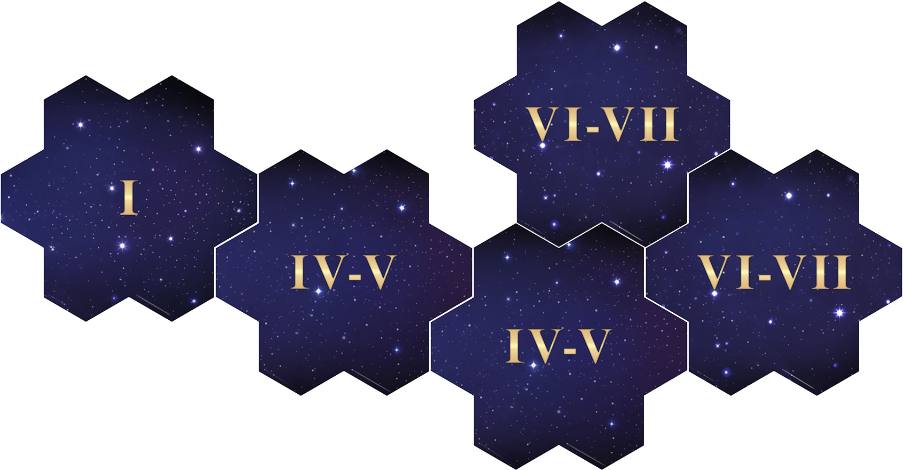
\includegraphics[width=0.45\textwidth]{\maps/gold_rush-solo.png}};
        \node at (14, 0) {\footnotesize{\textbf{SOLO VARIANT}}};
        \node at (4, -5) {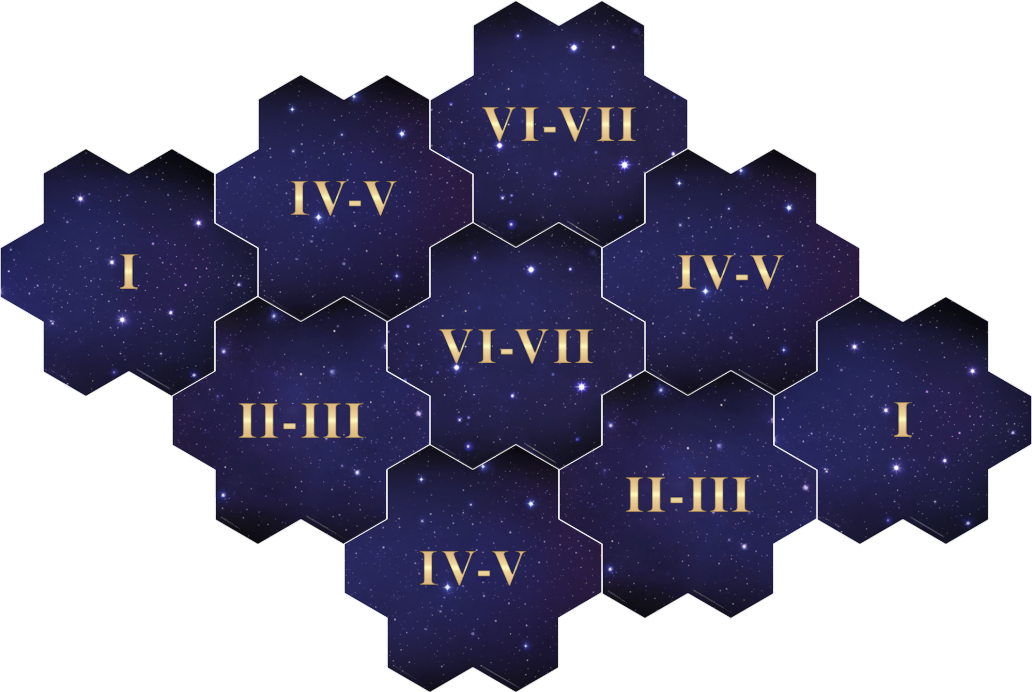
\includegraphics[width=0.48\textwidth]{\maps/gold_rush-1v1.png}};
        \node at (4, -9) {\footnotesize{\textbf{1v1 VARIANT}}};
        \node at (14, -6) {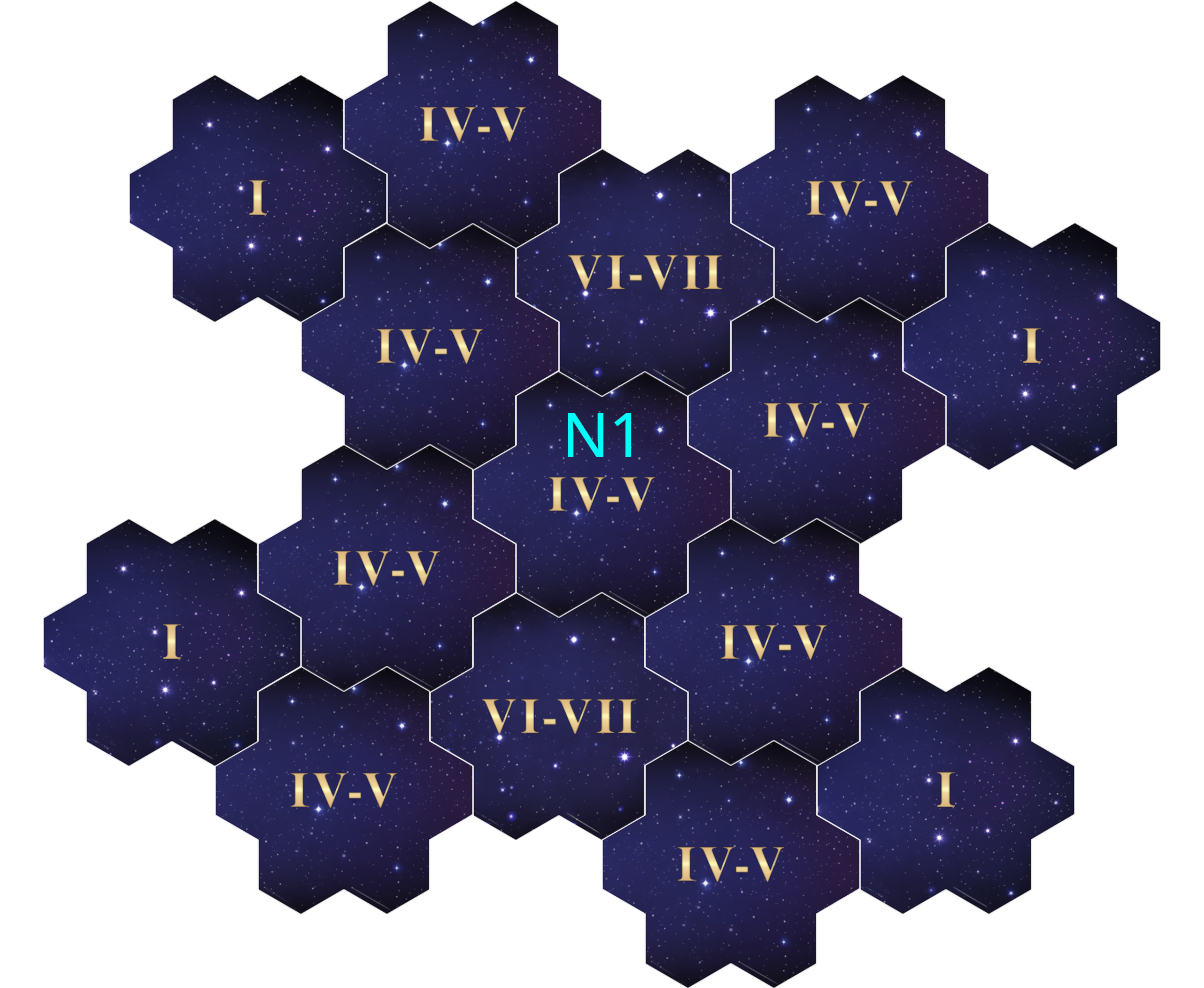
\includegraphics[width=0.56\textwidth]{\maps/gold_rush-2v2.png}};
        \node at (14, -11) {\footnotesize{\textbf{2v2 VARIANT}}};
    \end{tikzpicture}

\end{multicols*}
